\documentclass[]{article}
\usepackage{lmodern}
\usepackage{amssymb,amsmath}
\usepackage{ifxetex,ifluatex}
\usepackage{fixltx2e} % provides \textsubscript
\ifnum 0\ifxetex 1\fi\ifluatex 1\fi=0 % if pdftex
  \usepackage[T1]{fontenc}
  \usepackage[utf8]{inputenc}
\else % if luatex or xelatex
  \ifxetex
    \usepackage{mathspec}
  \else
    \usepackage{fontspec}
  \fi
  \defaultfontfeatures{Ligatures=TeX,Scale=MatchLowercase}
\fi
% use upquote if available, for straight quotes in verbatim environments
\IfFileExists{upquote.sty}{\usepackage{upquote}}{}
% use microtype if available
\IfFileExists{microtype.sty}{%
\usepackage{microtype}
\UseMicrotypeSet[protrusion]{basicmath} % disable protrusion for tt fonts
}{}
\usepackage[margin=1in]{geometry}
\usepackage{hyperref}
\hypersetup{unicode=true,
            pdftitle={R Learning Guide},
            pdfauthor={Mike Bader},
            pdfborder={0 0 0},
            breaklinks=true}
\urlstyle{same}  % don't use monospace font for urls
\usepackage{color}
\usepackage{fancyvrb}
\newcommand{\VerbBar}{|}
\newcommand{\VERB}{\Verb[commandchars=\\\{\}]}
\DefineVerbatimEnvironment{Highlighting}{Verbatim}{commandchars=\\\{\}}
% Add ',fontsize=\small' for more characters per line
\usepackage{framed}
\definecolor{shadecolor}{RGB}{248,248,248}
\newenvironment{Shaded}{\begin{snugshade}}{\end{snugshade}}
\newcommand{\KeywordTok}[1]{\textcolor[rgb]{0.13,0.29,0.53}{\textbf{{#1}}}}
\newcommand{\DataTypeTok}[1]{\textcolor[rgb]{0.13,0.29,0.53}{{#1}}}
\newcommand{\DecValTok}[1]{\textcolor[rgb]{0.00,0.00,0.81}{{#1}}}
\newcommand{\BaseNTok}[1]{\textcolor[rgb]{0.00,0.00,0.81}{{#1}}}
\newcommand{\FloatTok}[1]{\textcolor[rgb]{0.00,0.00,0.81}{{#1}}}
\newcommand{\ConstantTok}[1]{\textcolor[rgb]{0.00,0.00,0.00}{{#1}}}
\newcommand{\CharTok}[1]{\textcolor[rgb]{0.31,0.60,0.02}{{#1}}}
\newcommand{\SpecialCharTok}[1]{\textcolor[rgb]{0.00,0.00,0.00}{{#1}}}
\newcommand{\StringTok}[1]{\textcolor[rgb]{0.31,0.60,0.02}{{#1}}}
\newcommand{\VerbatimStringTok}[1]{\textcolor[rgb]{0.31,0.60,0.02}{{#1}}}
\newcommand{\SpecialStringTok}[1]{\textcolor[rgb]{0.31,0.60,0.02}{{#1}}}
\newcommand{\ImportTok}[1]{{#1}}
\newcommand{\CommentTok}[1]{\textcolor[rgb]{0.56,0.35,0.01}{\textit{{#1}}}}
\newcommand{\DocumentationTok}[1]{\textcolor[rgb]{0.56,0.35,0.01}{\textbf{\textit{{#1}}}}}
\newcommand{\AnnotationTok}[1]{\textcolor[rgb]{0.56,0.35,0.01}{\textbf{\textit{{#1}}}}}
\newcommand{\CommentVarTok}[1]{\textcolor[rgb]{0.56,0.35,0.01}{\textbf{\textit{{#1}}}}}
\newcommand{\OtherTok}[1]{\textcolor[rgb]{0.56,0.35,0.01}{{#1}}}
\newcommand{\FunctionTok}[1]{\textcolor[rgb]{0.00,0.00,0.00}{{#1}}}
\newcommand{\VariableTok}[1]{\textcolor[rgb]{0.00,0.00,0.00}{{#1}}}
\newcommand{\ControlFlowTok}[1]{\textcolor[rgb]{0.13,0.29,0.53}{\textbf{{#1}}}}
\newcommand{\OperatorTok}[1]{\textcolor[rgb]{0.81,0.36,0.00}{\textbf{{#1}}}}
\newcommand{\BuiltInTok}[1]{{#1}}
\newcommand{\ExtensionTok}[1]{{#1}}
\newcommand{\PreprocessorTok}[1]{\textcolor[rgb]{0.56,0.35,0.01}{\textit{{#1}}}}
\newcommand{\AttributeTok}[1]{\textcolor[rgb]{0.77,0.63,0.00}{{#1}}}
\newcommand{\RegionMarkerTok}[1]{{#1}}
\newcommand{\InformationTok}[1]{\textcolor[rgb]{0.56,0.35,0.01}{\textbf{\textit{{#1}}}}}
\newcommand{\WarningTok}[1]{\textcolor[rgb]{0.56,0.35,0.01}{\textbf{\textit{{#1}}}}}
\newcommand{\AlertTok}[1]{\textcolor[rgb]{0.94,0.16,0.16}{{#1}}}
\newcommand{\ErrorTok}[1]{\textcolor[rgb]{0.64,0.00,0.00}{\textbf{{#1}}}}
\newcommand{\NormalTok}[1]{{#1}}
\usepackage{longtable,booktabs}
\usepackage{graphicx,grffile}
\makeatletter
\def\maxwidth{\ifdim\Gin@nat@width>\linewidth\linewidth\else\Gin@nat@width\fi}
\def\maxheight{\ifdim\Gin@nat@height>\textheight\textheight\else\Gin@nat@height\fi}
\makeatother
% Scale images if necessary, so that they will not overflow the page
% margins by default, and it is still possible to overwrite the defaults
% using explicit options in \includegraphics[width, height, ...]{}
\setkeys{Gin}{width=\maxwidth,height=\maxheight,keepaspectratio}
\IfFileExists{parskip.sty}{%
\usepackage{parskip}
}{% else
\setlength{\parindent}{0pt}
\setlength{\parskip}{6pt plus 2pt minus 1pt}
}
\setlength{\emergencystretch}{3em}  % prevent overfull lines
\providecommand{\tightlist}{%
  \setlength{\itemsep}{0pt}\setlength{\parskip}{0pt}}
\setcounter{secnumdepth}{0}
% Redefines (sub)paragraphs to behave more like sections
\ifx\paragraph\undefined\else
\let\oldparagraph\paragraph
\renewcommand{\paragraph}[1]{\oldparagraph{#1}\mbox{}}
\fi
\ifx\subparagraph\undefined\else
\let\oldsubparagraph\subparagraph
\renewcommand{\subparagraph}[1]{\oldsubparagraph{#1}\mbox{}}
\fi

%%% Use protect on footnotes to avoid problems with footnotes in titles
\let\rmarkdownfootnote\footnote%
\def\footnote{\protect\rmarkdownfootnote}

%%% Change title format to be more compact
\usepackage{titling}

% Create subtitle command for use in maketitle
\newcommand{\subtitle}[1]{
  \posttitle{
    \begin{center}\large#1\end{center}
    }
}

\setlength{\droptitle}{-2em}
  \title{R Learning Guide}
  \pretitle{\vspace{\droptitle}\centering\huge}
  \posttitle{\par}
  \author{Mike Bader}
  \preauthor{\centering\large\emph}
  \postauthor{\par}
  \predate{\centering\large\emph}
  \postdate{\par}
  \date{February 2018}


\begin{document}
\maketitle

{
\setcounter{tocdepth}{3}
\tableofcontents
}
\section{Welcome to R!}\label{welcome-to-r}

You are embarking on an exciting adventure to learn extremely powerful
software that you can download \textbf{for free}.

\subsection{What is R?}\label{what-is-r}

Let's start by describing this powerful tool to start. R is both:

\begin{itemize}
\item
  A statistical computing software
\item
  A full-fledged programming language
\end{itemize}

If you have learned other statistical software, you might wonder why you
would want to learn another. Especially because many find that R has a
steeper learning curve than these software programs.

\subsection{Difference from Other Statistical
Software}\label{difference-from-other-statistical-software}

Other statistical software like Stata, SPSS, and SAS do one thing: they
take a table (spreadsheet) of data and statistical commands to analyze
that data.

R can do this, too. But R can do many more things because R is an entire
programming language. It has many different types of data that you can
use. You can put in a table (called a ``data frame'' in R-speak), but
you have lots of other types of data that you can use. It offers much
more flexibility than other statistical software.

BUT, that flexibility comes at the cost of simplicity.

\subsection{Why R?}\label{why-r}

So why make you learn something that's harder than what you have already
learned?

\begin{itemize}
\item
  R is open source (free as in speech), which means that many different
  people can help extend the language to do common tasks or specialized
  analysis
\item
  R is the future of statistical software; employers will be
  increasingly moving to R
\item
  Lest we forget, let us remember that R is \textbf{free} (as in beer);
  you can use it on any computer and with any employer. Many of you will
  be working for employers that might not have large budgets; learning
  free software means that you will always be able to use it.

  \begin{longtable}[]{@{}lrl@{}}
  \toprule
  SAS\footnote{For SAS Analytics Pro
    \url{https://www.sas.com/en_us/software/analytics-pro.html}; January
    20, 2018} & \$9,720.00 & + Windows only\tabularnewline
  SPSS\footnote{\url{https://www.ibm.com/products/spss-statistics/pricing};
    January 20, 2018} & \$99.00/month & + \$237.00/month
  add-ons\tabularnewline
  Stata\footnote{Stata 15 government \& nonprofit pricing
    \url{https://www.stata.com/order/new/gov/single-user-licenses/dl/};
    January 20, 2018} & \$1,695.00 & + \$300 for large
  datasets\tabularnewline
  R & \$0.00 &\tabularnewline
  \bottomrule
  \end{longtable}
\end{itemize}

We're talking about a substantial amount of money!

\section{Getting R}\label{getting-r}

\subsection{Download R}\label{download-r}

I hope that I have convinced you to at least try R at this point. That
means you will need to get this amazing, powerful, and cost-effective
software. You will need to download R. To do so Go to
\url{https://www.r-project.org/} and look for the link that says
``Download.'' After you do that, you will be sent to a list of mirrors
(servers that distribute R so that no single server gets overloaded).
Find the United States and download one from that lists (I use the
\href{https://mirrors.nics.utk.edu/cran/}{National Institute for
Computational Sciences in Oak Ridge, TN}).

\subsection{RStudio}\label{rstudio}

If you open up R after downloading it, you will see that it gives you
\emph{nothing} except a command line to type in commands to be run. This
is not ideal and would make R \emph{really} difficult if that was the
only way with which you could interact with R.

That is where RStudio comes in. RStudio is an \emph{Integrated
Development Environment (IDE)} for R. That means that RStudio gives you
a window into R--basically it acts as a gopher between you and R.

In acting as a gopher, it provides a nice \emph{graphical user interface
(GUI)} that makes R a lot easier to use.

There are four different windows in RStudio that you will use:

\begin{description}
\item[Source (ctrl-1)]
This is where you keep your scripts where you do your analysis. These
are the same as {\texttt{.do}} files in Stata.
\item[Console (ctrl-2)]
This is where you can type commands directly to tell R what to do. You
should use this sparingly because only entering commands in the console
makes it difficult to reproduce what you have done. My advice: work in
the source window, then copy/paste into the console (or source the
command directly by pressing `ctrl-Enter'---we'll get to that)
\item[Environment]
This window shows you all of the objects that are currently available in
R. Remember how I told you that R can hold different types of data? This
is where you will find all of them. A second tab in that window contains
your history, which contains the list of commands that you have entered
into the console.
\item[Viewer]
This window is where you will view help files and plots that you make
(you can view a whole bunch of other stuff down there, but those are for
more advanced applications).
\end{description}

To get RStudio, you will go to \url{https://www.rstudio.com/} and then
find the link for RStudio and download. This software is also free.

\subsection{Getting Help}\label{getting-help}

As you go on this adventure, you will likely need help along the way.
There are a couple of great resources on the web to help you learn just
about everything that you would like to do.

\begin{description}
\item[\href{https://stackoverflow.com/questions/tagged/r}{Stack
Overflow}]
provides user-generated answers to questions posed in forums. Good
answers tend to filter to the top of the list based on an ingenuous
ranking system of votes and points.
\item[\href{https://rseek.org/}{Rseek}]
gives Google-like search functionality to find R-related material.
\item[\href{https://www.r-bloggers.com/}{R-bloggers}]
is a blog with posts that cover tutorials and code for basic to advanced
material
\end{description}

\section{First Steps with R}\label{first-steps-with-r}

\subsection{What is a Variable?}\label{what-is-a-variable}

In R, \emph{variables} differ from variables in other statistics
programs. In Stata or SPSS, variables represent columns in a dataset. In
R, variables can take on many different forms: vectors (a row of numbers
or letters), datasets (called ``dataframes''), scalars (a single number
or letter), among many others
(\href{https://www.statmethods.net/input/datatypes.html}{here} is a list
of different R objects).

\hypertarget{vars_numeric}{\subsubsection{Numeric}\label{vars_numeric}}

We will ``assign'' variables in R using the operator
\texttt{\textless{}-}. If we want to create a variable containing the
number of states in the United States (50) to a variable named
\texttt{N\_states} for {[}N{]}umber of {[}states{]}\footnote{R reads
  periods \texttt{.} as spaces, like underscores. Those who code in
  Python will likely find this convention frustrating since Python uses
  the dot notation to identify methods or properties of an object's
  instance. In my own coding, I now try to use underscores rather than
  dots so that I do not continue to confuse myself, even though dots are
  conventional in R.} we might write:

\begin{Shaded}
\begin{Highlighting}[]
\NormalTok{N_states <-}\StringTok{ }\DecValTok{50}
\end{Highlighting}
\end{Shaded}

Any time we write \texttt{N\_states}, R will read that as ``50''. So if
I type \texttt{N\_states\ *\ 2} into the console, I will get:

\begin{Shaded}
\begin{Highlighting}[]
\NormalTok{N_states *}\StringTok{ }\DecValTok{2}
\end{Highlighting}
\end{Shaded}

\begin{verbatim}
## [1] 100
\end{verbatim}

\hypertarget{vars_string}{\subsubsection{Strings}\label{vars_string}}

We can also assign strings, or in R-speak ``characters'', to variables.
I can create a variable called \texttt{my\_state} that contains the
string \texttt{Maryland} in it. We can then do things with that variable
like make parts of sentences.

\begin{Shaded}
\begin{Highlighting}[]
\NormalTok{my_state <-}\StringTok{ "Maryland"}
\KeywordTok{paste}\NormalTok{(}\StringTok{"I live in"}\NormalTok{,my_state)}
\end{Highlighting}
\end{Shaded}

\begin{verbatim}
## [1] "I live in Maryland"
\end{verbatim}

Here we have used the \texttt{paste()} \emph{function} to glue the
string \texttt{"I\ live\ in"} to the string stored in
\texttt{my\_state}, which R reads as \texttt{"Maryland"}. If you wanted
to change the value in your state, you would only need to change the
value of \texttt{my\_state}, enclosed in quotes, to represent your
state. As a matter of fact, you don't even need to enter a state into
the variable \texttt{my\_state}, you can enter any value you want. For
example:

\begin{Shaded}
\begin{Highlighting}[]
\NormalTok{my_state <-}\StringTok{ "a galaxy far, far away"}
\KeywordTok{paste}\NormalTok{(}\StringTok{"I live in"}\NormalTok{,my_state)}
\end{Highlighting}
\end{Shaded}

\begin{verbatim}
## [1] "I live in a galaxy far, far away"
\end{verbatim}

This works because R doesn't care what string \texttt{my\_state}
actually contains. Now that I have entered
\texttt{"a\ galaxy\ far,\ far\ away"}, R will just look for the name
\texttt{my\_state} and substitute the value stored in that variable. You
should note that \emph{variable names are for humans} to make sense of
what's contained within them. R does not care what you name a variable,
it just cares what you assign to the variable of that name.

\textbf{Watch out:} One common error is to forget to enclose words in
quotes that you want to use as strings. R will ``throw'' an error if you
type the following:

\begin{Shaded}
\begin{Highlighting}[]
\NormalTok{my_state <-}\StringTok{ }\NormalTok{Maryland}
\end{Highlighting}
\end{Shaded}

\begin{verbatim}
## Error in eval(expr, envir, enclos): object 'Maryland' not found
\end{verbatim}

You will see that the console tells you ``Error: object `Maryland' not
found''. That means that R looked for a variable (that's the object its
referring to) called \texttt{Maryland}, but it couldn't find one. In
order for the string of letter M-a-r-y-l-a-n-d to be read as the string
``Maryland'', you need to enclose it in quotes.

\hypertarget{vars_vector}{\subsubsection{Vectors}\label{vars_vector}}

Vectors are another useful type of object in R. We create these by
``combining'' elements, separated by commas, into a single object. One
of the most annoying aspects of R is that you must use a function,
\texttt{combine()} to create vectors. Fortunately, because we use that
function so often, it has an abbreviation: \texttt{c()}.\footnote{For
  those unfamiliar with other programming languages, this might not seem
  weird. For those of us who program in other languages, for example
  Python, we get used to typing \texttt{my\_list\ =\ {[}1,2,3,4{]}}.
  Creating a similar object in R requires that we type
  \texttt{my\_list\ =\ c(1,2,3,4)}. I usually introduce errors in my
  code when I switch back to R from another language because I try to
  type \texttt{my\_list\ =\ (1,2,3,4)} and end up with an error.} Let's
say that I want to create a vector containing the states in which I have
lived. I would write:

\begin{Shaded}
\begin{Highlighting}[]
\NormalTok{my_states <-}\StringTok{ }\KeywordTok{c}\NormalTok{(}\StringTok{"Colorado"}\NormalTok{,}\StringTok{"Washington"}\NormalTok{,}\StringTok{"Maryland"}\NormalTok{,}\StringTok{"Texas"}\NormalTok{,}
               \StringTok{"Michigan"}\NormalTok{,}\StringTok{"New York"}\NormalTok{,}\StringTok{"Pennsylvania"}\NormalTok{)}
\end{Highlighting}
\end{Shaded}

Anytime I type \texttt{my\_states}, it will return the vector containing
this set of string values. With a ``for loop'' we could do the following
(don't worry about following the for-loop, just see that I can operate
on each element of the vector):

\begin{Shaded}
\begin{Highlighting}[]
\NormalTok{for(state in my_states) \{}
    \KeywordTok{print}\NormalTok{(}\KeywordTok{paste}\NormalTok{(}\StringTok{"I lived in"}\NormalTok{,state))}
\NormalTok{\}}
\end{Highlighting}
\end{Shaded}

\begin{verbatim}
## [1] "I lived in Colorado"
## [1] "I lived in Washington"
## [1] "I lived in Maryland"
## [1] "I lived in Texas"
## [1] "I lived in Michigan"
## [1] "I lived in New York"
## [1] "I lived in Pennsylvania"
\end{verbatim}

Note that when I initialized the variable \texttt{my\_states}, I split
the code across two lines. Normally R would execute each line as a
command. R, however, allows you to split lines inside of parentheses and
it won't attempt to execute the command until it finds the closing
parens. This allows you to keep your code in a reasonable width, which
improves legibility (generally try to keep each line under 80 characters
in width).

\subsection{Open a Dataset}\label{open-a-dataset}

None of this provides much excitement. After all, if you are reading
this tutorial, you likely want to analyze data. In order to analyze
data, we need to open a dataset to analyze.

\textbf{Data frames.} Remember that R stores every object with a
variable name: this includes datasets! As I mentioned above, R names
datasets ``data frames''. That means that we will load the data into a
variable and then operate on that variable to do things with the data.
This differs substantially from Stata or SPSS where you will load a
single data set and then the software will assume that you are refering
to that dataset when you send commands to the program.

For this example, we will use data from the 2016 DC Area Survey
(DCAS2016), a survey of residents in multiracial neighborhoods in
Washington, DC and the surrounding jurisdictions. The data are available
at
\url{https://hg.mikebader.net/private/dcas2016/raw-file/tip/Dataset/DCAS_2016_weighted.csv}
(email me to get the username and password if you would like to download
the data).

The file contains the data in \emph{comma separated values (csv)}
format. The first row contains ``variable'' (in the sense of data
variables, not in the R sense) names separated by commas. Each of the
following rows contains the responses for a single respondent with each
reponse separated by a comma.

Comma separated values can always be read, which gives them a huge
advantage over files saved in a format that cannot be read. It's like
saving a text file on your computer versus a Microsoft Word document. It
seems fine because of Word's ubiquity. But I'm old enough to remember
when WordPerfect was the word processor that everyone used. Good luck
getting one of those files to open now.

I digress. We have two options for data that are available on the web:
we can download the data and open the file from our machine or we can
open the data directly from the internet. My advice would be this: if
you a dataset will not change, then download a copy so that you can use
it at any time. If a dataset will change, for example by getting new
data appended as they become available, it's probably better to open the
data from the internet.

\hypertarget{data_local}{\subsubsection{\texorpdfstring{Loading data
from a file on your computer (also known as loading from a `local
file').}{Loading data from a file on your computer (also known as loading from a local file).}}\label{data_local}}

To be able to open the data, you will have to tell R where you have
stored it on your computer. To do this, you will need to know a) the
directory in which you stored it and b) the file name. Every operating
system stores files into different directories. You probably know these
as folders when you go to ``My Computer'' on a PC or ``Macintosh HD'' on
a Mac (if you use Linux, I will assume that you know all of this and you
can probably tell me how I've gotten this wrong). The folders just
provide a visual representation of directories.

To open the data, you will use the function \texttt{read.csv()}. The
function takes one required \emph{argument}, the file name to be read. R
will then convert the text in the .csv file into a dataframe that we can
manipulate and analyze. Remember, though, that \emph{we need to assign
the dataset to a variable in R!} I downloaded my data into a drive
called ``\textasciitilde{}/work/Data/DCAS/dcas2016/sourceData/'' and I
kept the original file name, ``DCAS\_2016\_weighted.csv'', and want to
store the data in an object called \texttt{dcas}. So, I would write:

\begin{Shaded}
\begin{Highlighting}[]
\NormalTok{dcas <-}\StringTok{ }\KeywordTok{read.csv}\NormalTok{(}\StringTok{"~/work/Data/DCAS/dcas2016/Dataset/DCAS_2016_weighted.csv"}\NormalTok{)}
\end{Highlighting}
\end{Shaded}

Let's break what we did here into its parts:

\begin{itemize}
\item
  {\texttt{dcas}}\\
  This is the object that holds the dataset that we read from the file.
  If we ever want to refer to the dataset, we would need to reference
  its name, {\texttt{dcas}}, first. One of the really cool things about
  R is that you can have multiple datasets open at the same time; that
  means, however, that you have to refer to the dataset that you want to
  use by its name.
\item
  {\texttt{\textless{}-}}\\
  Just as with the variables above, this means ``assign'' the contents
  of the file to the variable name \texttt{dcas}.
\item
  {\texttt{read.csv()}}\\
  This is the \emph{function}. You can tell that it is a function
  because it has parentheses after it. Inside the parentheses are
  different \emph{arguments} that you pass to the function. A function
  will then take those options and do something with them.
\item
  {\texttt{"\textasciitilde{}/work/Data/DCAS/dcas2016/Dataset/DCAS\_2016\_weighted.csv"}}\\
  is a file that holds the data that we want. Notice that we must put
  the file name in quotations. Otherwise R would look for an object of
  the name
  \texttt{\textasciitilde{}/work/Data/DCAS/dcas2016/Dataset/DCAS\_2016\_weighted.csv}
  (which would fail miserably).
\end{itemize}

R did not complain to us, so that's a good sign. But, the data might not
have loaded correctly, so I always like to check. You can do this in two
ways if you are using RStudio. The first, and my preferred way, to check
the data is to use the \texttt{View()} function, which will show you the
contents of the object in the source window.

\begin{Shaded}
\begin{Highlighting}[]
\KeywordTok{View}\NormalTok{(dcas)}
\end{Highlighting}
\end{Shaded}

You can see the result of the \texttt{View(dcas)} command in the source
pane (top left pane) in the image below. The data appear to be set up
correctly. The data's variables are listed across the top, the actual
values in the cells. Everything looks good!

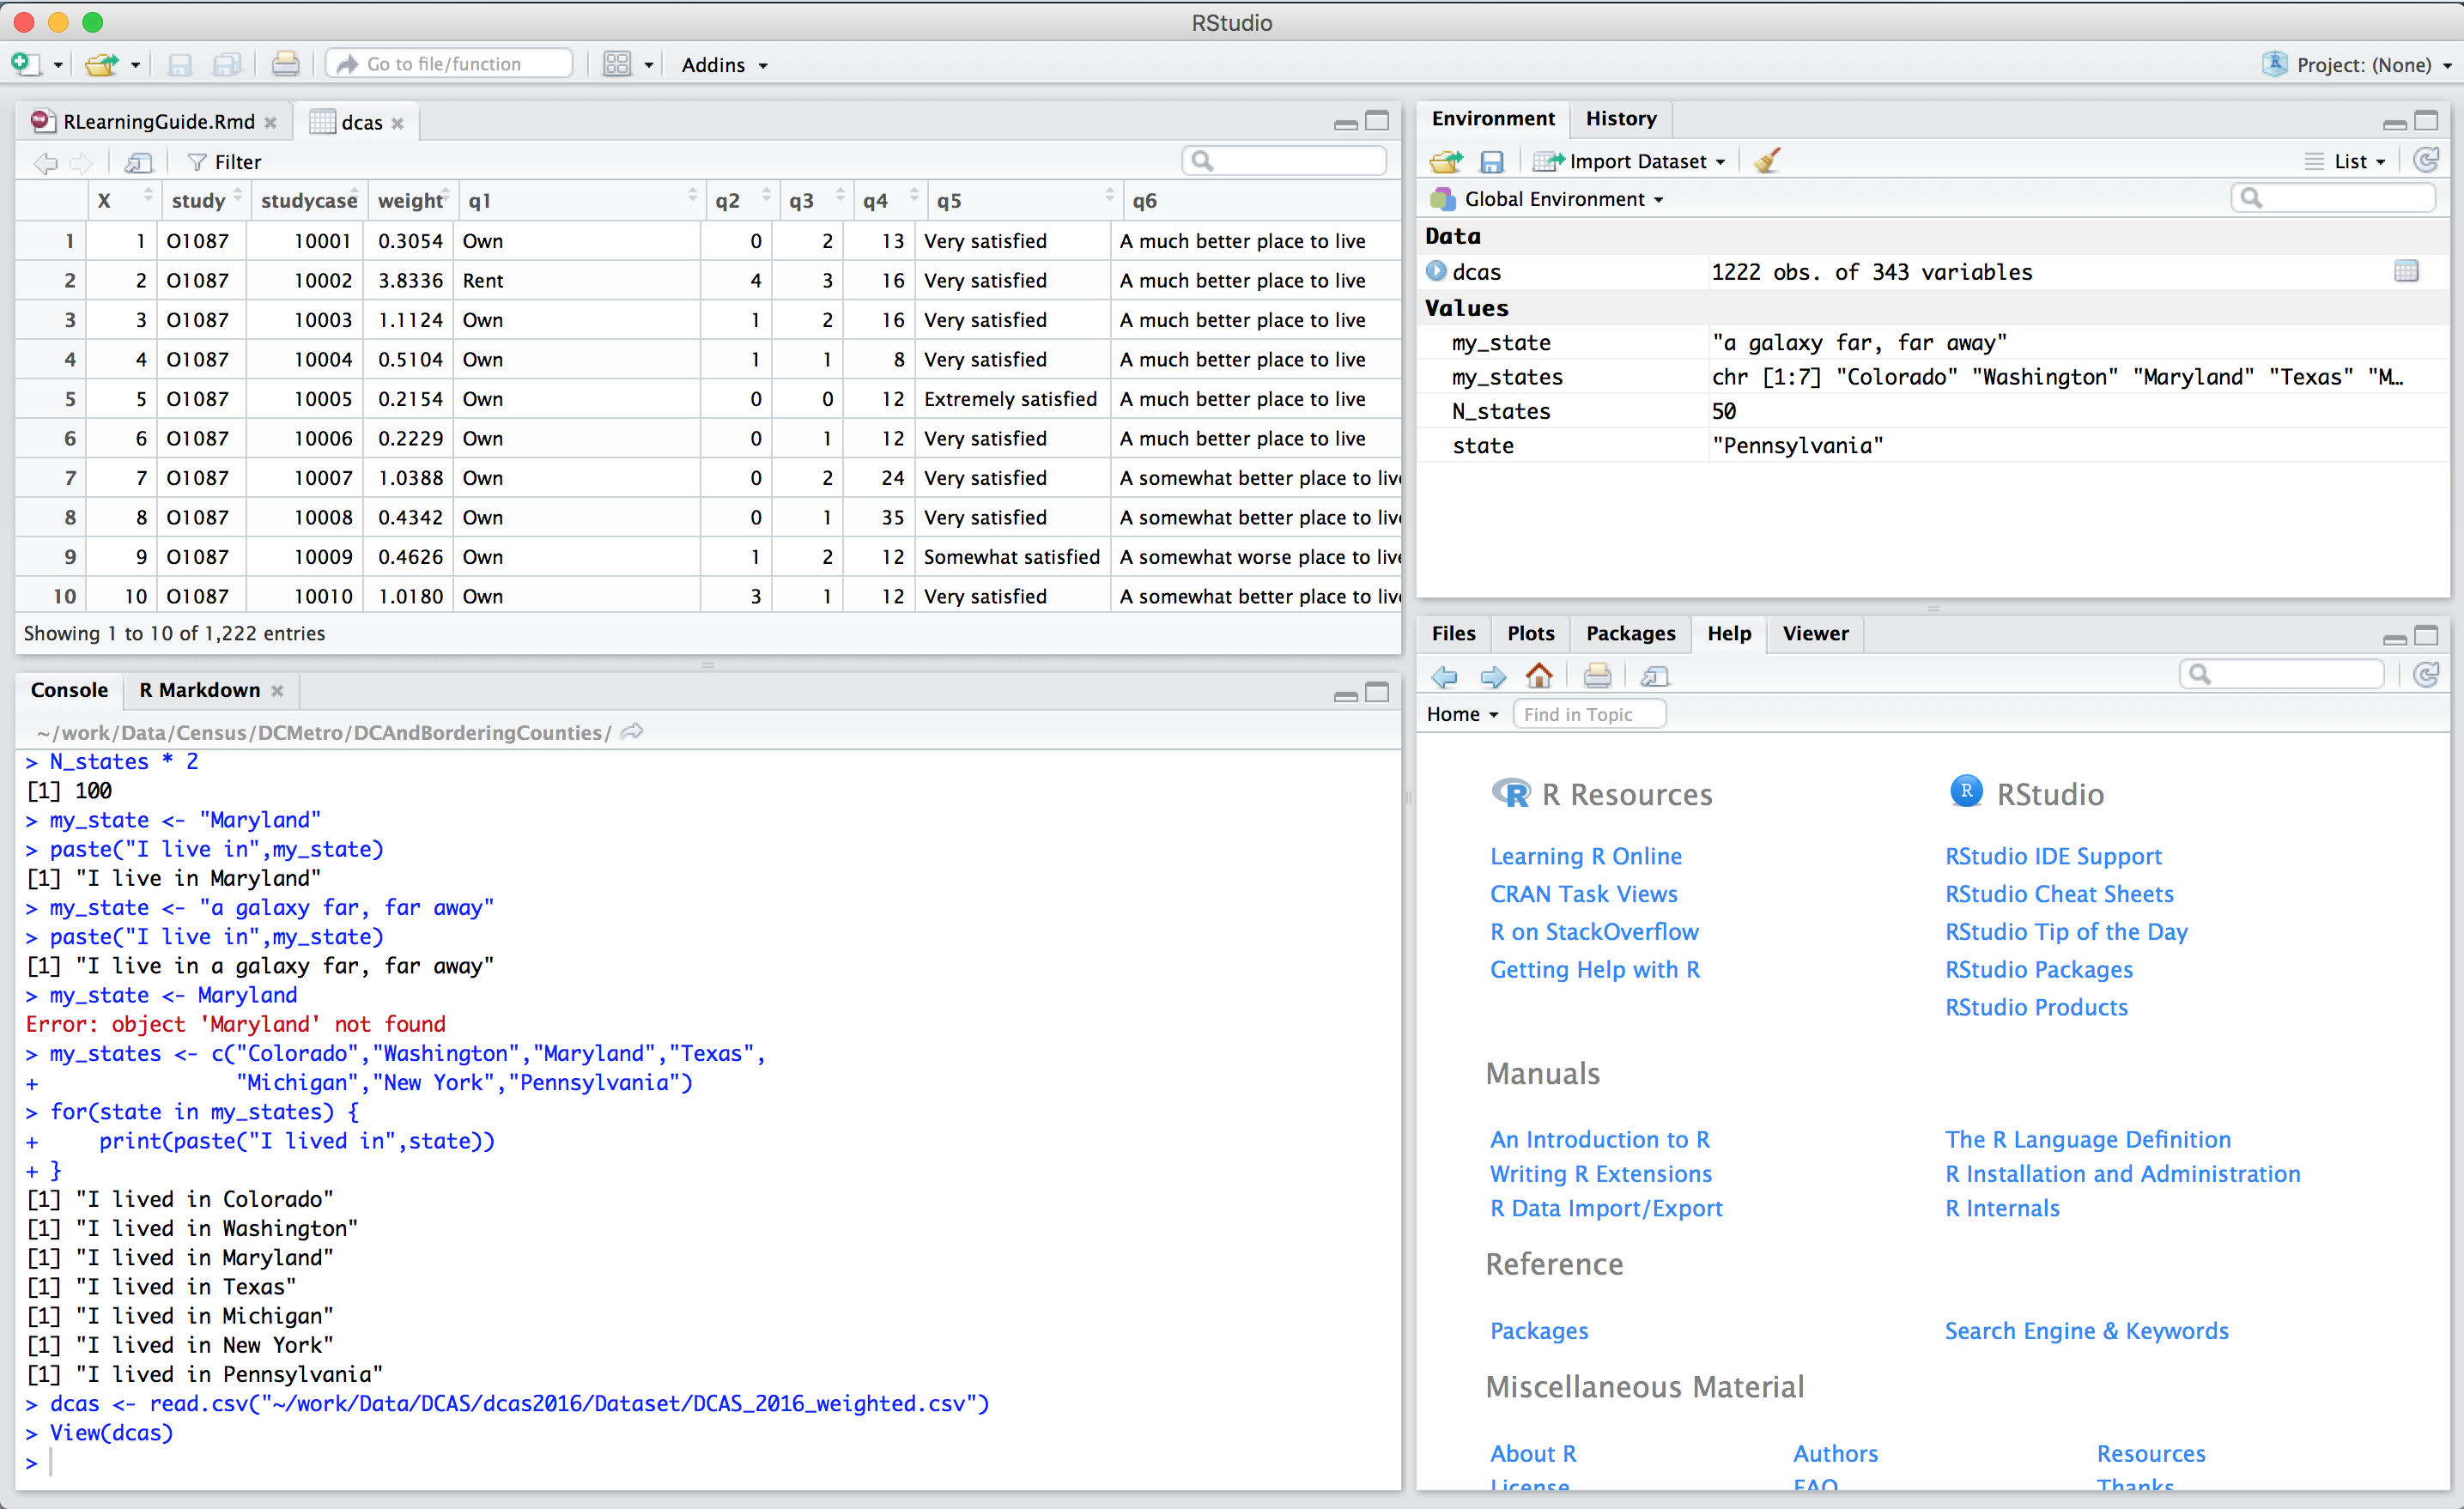
\includegraphics[width=5in]{images/View_function_screenshot}

The \texttt{head()} function provides another way to check the data.
This works whether or not you are using RStudio. The \texttt{head()}
function takes one required argument, the data frame object. By default
it will show you the first six rows of data. You can add an extra
argument, however, to tell it how many rows you want reported.

Although most R tutorials and resources tell you to use \texttt{head()},
I don't find it useful because it prints so much data, it can be very
difficult to read. Below, I will show you what the data look like
including only the first 15 columns of the data. If you would like to
see the full results in all of their ugliness, you can type
\texttt{head(dcas)} rather than what I have here. Just remember, I
warned you!

\begin{Shaded}
\begin{Highlighting}[]
\KeywordTok{head}\NormalTok{(dcas[,}\KeywordTok{c}\NormalTok{(}\DecValTok{1}\NormalTok{:}\DecValTok{15}\NormalTok{)])}
\end{Highlighting}
\end{Shaded}

\begin{verbatim}
##   X study studycase weight   q1 q2 q3 q4                  q5
## 1 1 O1087     10001 0.3054  Own  0  2 13      Very satisfied
## 2 2 O1087     10002 3.8336 Rent  4  3 16      Very satisfied
## 3 3 O1087     10003 1.1124  Own  1  2 16      Very satisfied
## 4 4 O1087     10004 0.5104  Own  1  1  8      Very satisfied
## 5 5 O1087     10005 0.2154  Own  0  0 12 Extremely satisfied
## 6 6 O1087     10006 0.2229  Own  0  1 12      Very satisfied
##                            q6              q7              q8
## 1 A much better place to live   1 to 4 blocks   Very unlikely
## 2 A much better place to live   5 to 9 blocks   Very unlikely
## 3 A much better place to live 10 to 25 blocks   Very unlikely
## 4 A much better place to live   5 to 9 blocks Somewhat likely
## 5 A much better place to live   5 to 9 blocks     Very likely
## 6 A much better place to live   1 to 4 blocks   Very unlikely
##                                       q9 q10_1 q10_2
## 1     Become a much better place to live  Some A few
## 2  Become a somewhat worse place to live A few  None
## 3                  Stayed about the same  None  None
## 4                  Stayed about the same  Most  None
## 5     Become a much better place to live A few A few
## 6 Become a somewhat better place to live  None  None
\end{verbatim}

\hypertarget{data_internet}{\subsubsection{Loading Data from the
Internet}\label{data_internet}}

The other option you have to read data into R is to read it directly
from the internet. In this case, you will pass the URL where the data
are stored to the \texttt{read.csv()} file rather than a file in a local
directory. As I mentioned above, this feature might be especially good
for data that are updated regularly.

Zillow provides one such source of data. On their
\href{https://www.zillow.com/research/data/}{research data page}, Zillow
provides a number of time series datasets that they update either every
quarter or every month. One could use these updated data to track trends
and automatically get the most recent results available by downloading
from the web.

The data that I will use for this example uses Zillow's proprietary
\href{https://wp.zillowstatic.com/3/ZHVI-InfoSheet-04ed2b.pdf}{Home
Value Index (ZHVI)} because it contains estimates over many years for
most US metropolitan areas. The file is located at:
\url{http://files.zillowstatic.com/research/public/Metro/Metro_Zhvi_AllHomes.csv}.

Therefore, we will download the data by passing that URL to the
\texttt{read.csv()} function rather than a file on our own computer
(remember the put the URL in quotes).

\begin{Shaded}
\begin{Highlighting}[]
\NormalTok{zillow <-}\StringTok{ }\KeywordTok{read.csv}\NormalTok{(}\StringTok{"http://files.zillowstatic.com/research/public/Metro/Metro_Zhvi_AllHomes.csv"}\NormalTok{)}
\end{Highlighting}
\end{Shaded}

Now it would be wise to inspect the data, either by using
\texttt{View(zillow)} in RStudio or \texttt{head(zillow)}.\footnote{If
  you inspect it closely, you will see that the first row contains data
  for the entire US rather than an individual metropolitan area. If you
  wanted to use these data to compare metropolitan areas, then you would
  want to remove that row before any analysis. We will discuss how to do
  that later in this Guide.}

\section{Review}\label{review}

\begin{itemize}
\tightlist
\item
  R provides a versatile, powerful set of tools for free (as in beer)
  with a large and stable user base that can contribute to the
  development (free as in speech)
\item
  R can (and does) store all types of objects into variables, including
  \protect\hyperlink{vars_numeric}{numeric},
  \protect\hyperlink{vars_string}{strings}, and
  \protect\hyperlink{vars_vector}{vectors}
\item
  You must load data into an object and can do so by either downloading
  data and loading it \protect\hyperlink{data_local}{from your local
  machine} or from the \protect\hyperlink{data_internet}{internet}.
\end{itemize}


\end{document}
